\section{Мета роботи}
Освоєння аналітичних методів аналізу трудомісткості
обчислювальних алгоритмів.

\section{Хід роботи}
1) З табл. 1.2 обрати логічну схему алгоритму (ЛСА) відповідно до
варіанта.
\begin{figure}[h]
    \centering
    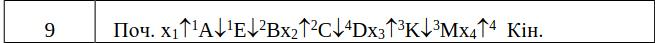
\includegraphics[width=16cm]{reports/algos/lab1/assets/1.png}
\end{figure}

З табл. 1.3 вибрати ймовірності переходів при одиничних логічних
умовах.
\begin{figure}[h]
    \centering
    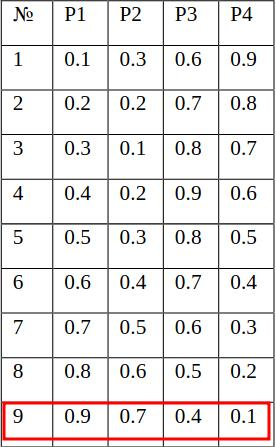
\includegraphics[width=8cm]{reports/algos/lab1/assets/2.png}
\end{figure}


\clearpage
2) За ЛСА побудувати графічну схему алгоритму, граф алгоритму та
мінімальний граф алгоритму.
\begin{figure}[h]
    \vspace{20mm} 
    \centering
    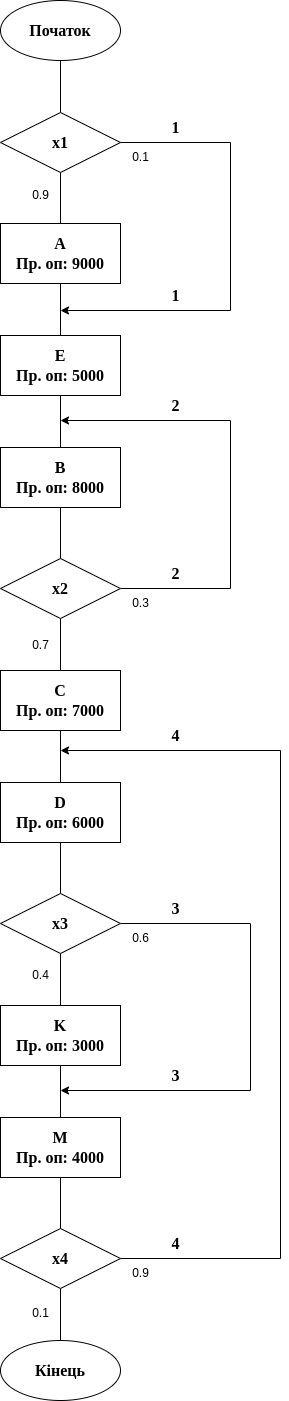
\includegraphics[width=0.2\textwidth]{reports/algos/lab1/assets/3.jpg}
    \caption{графічна схема}
\end{figure}

\begin{figure}[h]
    \centering
    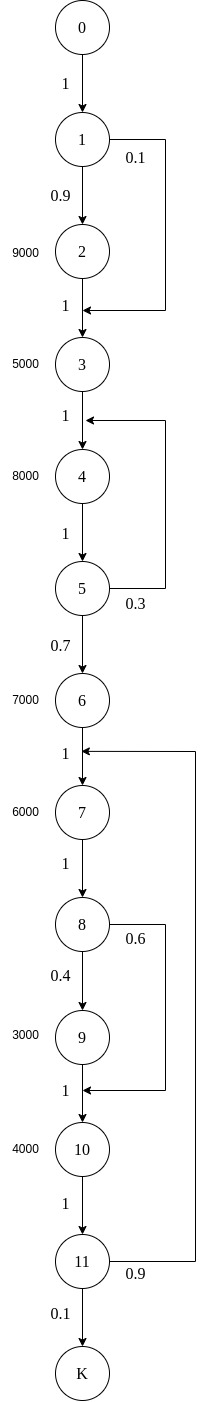
\includegraphics[width=0.2\textwidth]{reports/algos/lab1/assets/4.jpg}
    \caption{граф алгоритму}
\end{figure}

\begin{figure}[h]
    \centering
    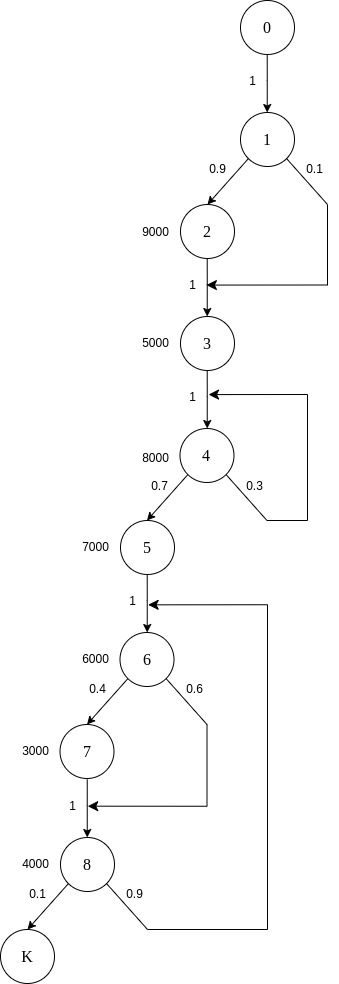
\includegraphics[width=8cm]{reports/algos/lab1/assets/5.jpg}
    \caption{мінімальний граф алгоритму}
\end{figure}

\clearpage
3) Визначити трудомісткість алгоритму методами \textbf{теорії марковських ланцюгів}.
\begin{figure}[h]
    \vspace{10mm} 
    \centering
    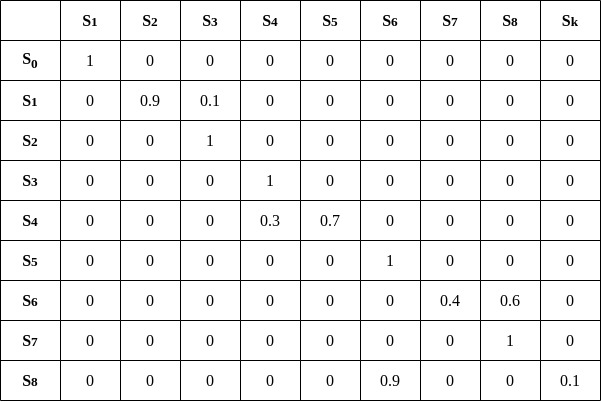
\includegraphics[width=14cm]{reports/algos/lab1/assets/6.jpg}
    \caption{Стохастична матриця алгоритму}
\end{figure}

\begin{figure}[h] 
    \centering
    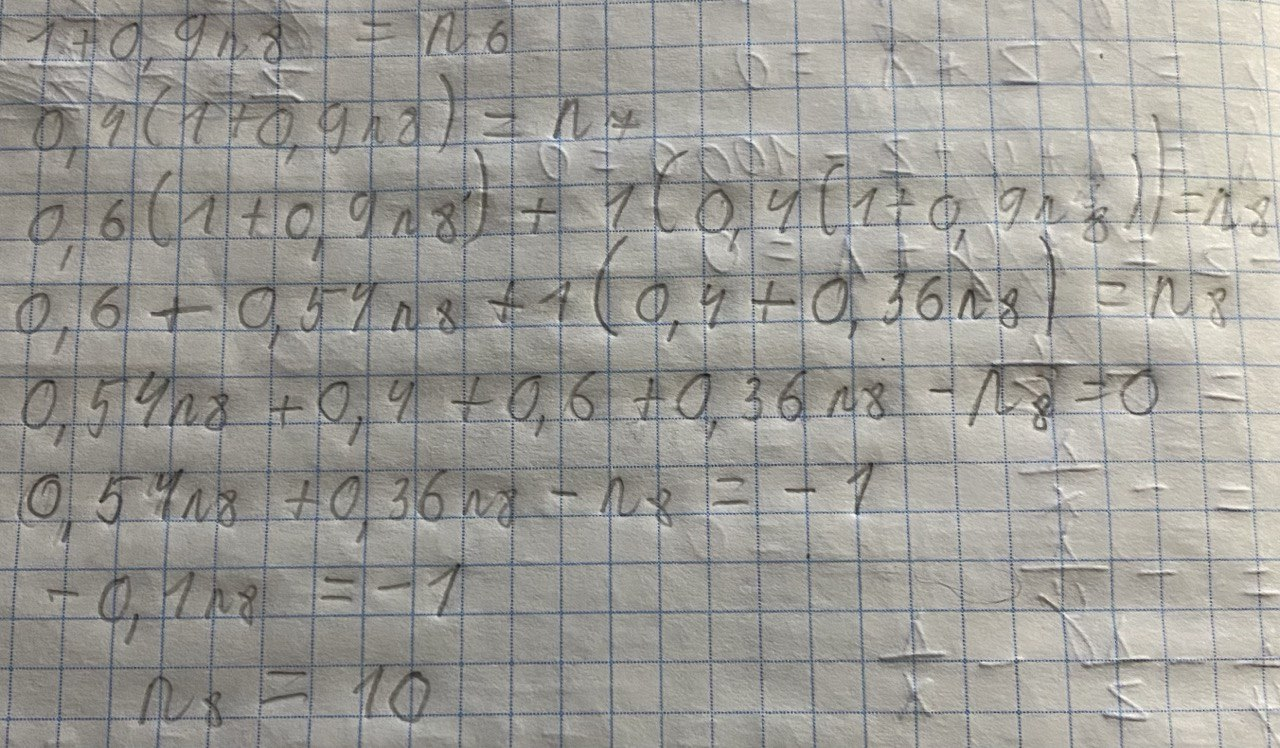
\includegraphics[width=11cm]{reports/algos/lab1/assets/8.jpg}
    \caption{Обчислення кількості звертань до усіх вершин графа}
\end{figure}

\begin{figure}[h]
    \centering
    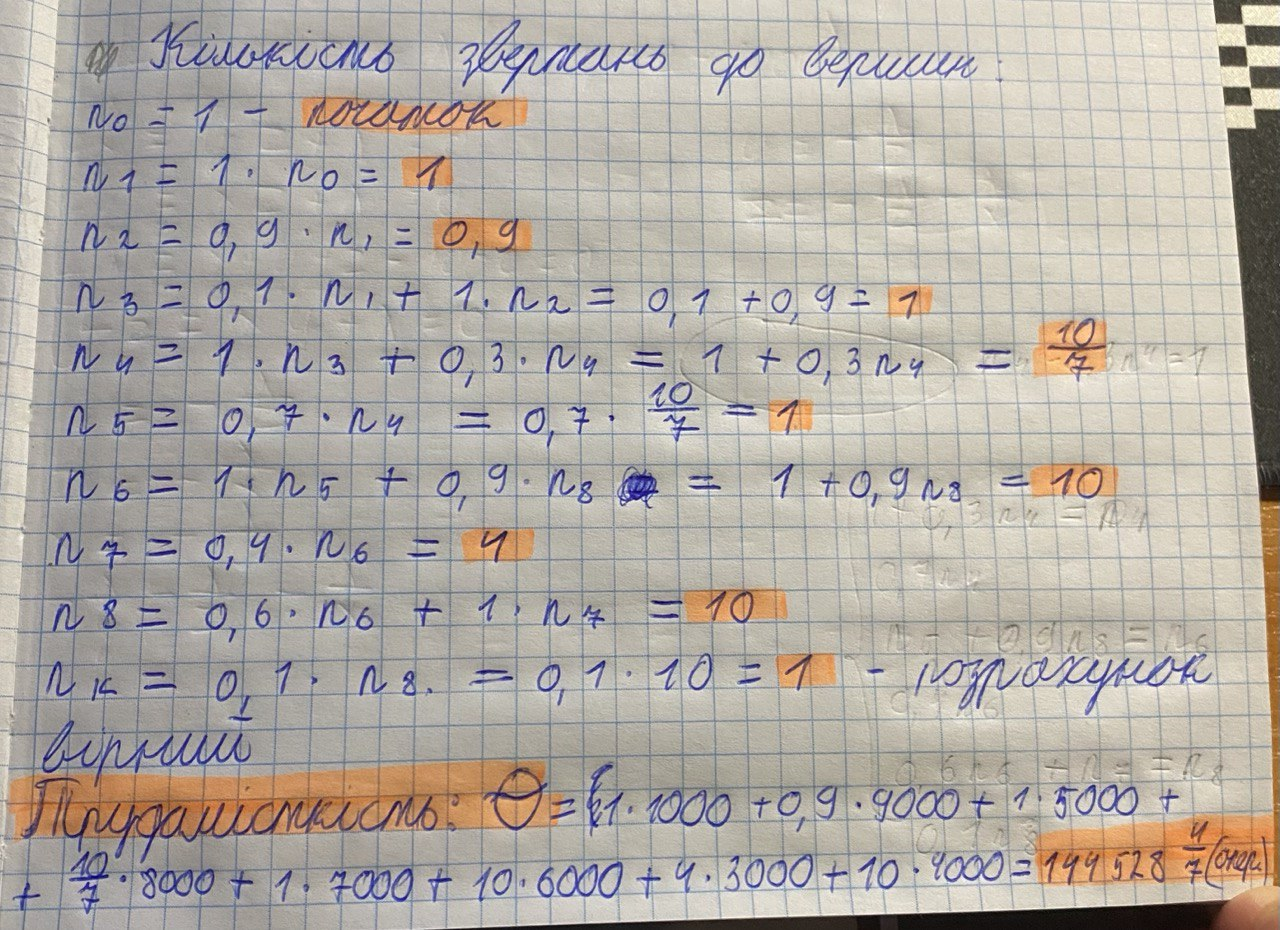
\includegraphics[width=16cm]{reports/algos/lab1/assets/7.jpg}
    \caption{Обчислення кількості звертань до усіх вершин графа та його трудомісткості}
\end{figure}

\clearpage
4) Визначити трудомісткість алгоритму \textbf{мережевим методом}.

\begin{figure}[h!]
    \centering
    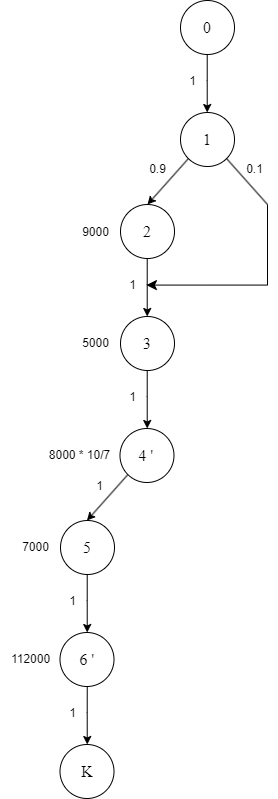
\includegraphics[width=8cm]{reports/algos/lab1/assets/9.png}
    \caption{Спрощений граф зі злитими циклами у одну вершину}
\end{figure}

\begin{figure}[h!]
    \centering
    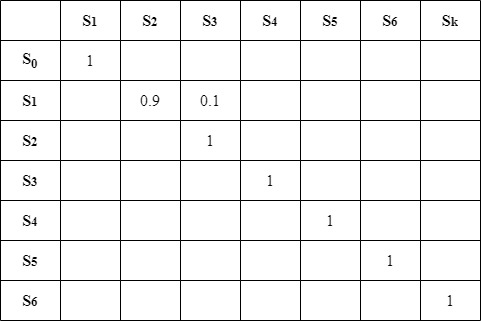
\includegraphics[width=14cm]{reports/algos/lab1/assets/10.jpg}
    \caption{Стохастична матриця алгоритму}
\end{figure}

\begin{figure}[h!]
    \centering
    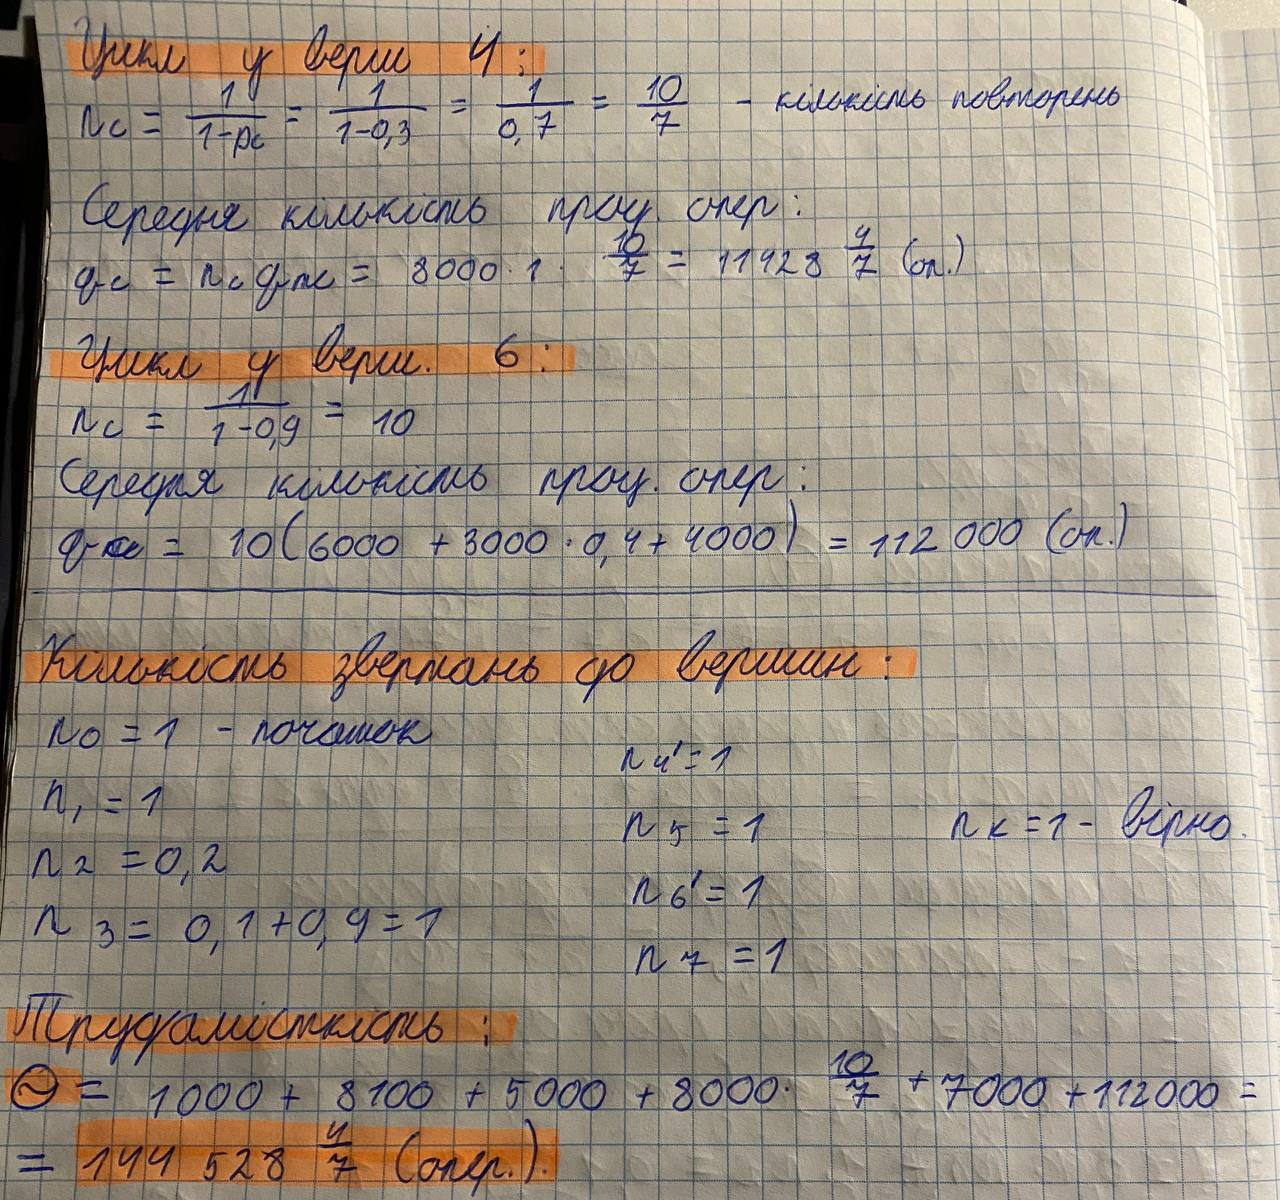
\includegraphics[width=14cm]{reports/algos/lab1/assets/11.jpg}
    \caption{Обчислення кількості звертань до усіх вершин графа та його трудомісткості}
\end{figure}

\clearpage
5) Обчислити мінімальну і максимальну трудомісткість алгоритму.

\begin{figure}[h!]
    \centering
    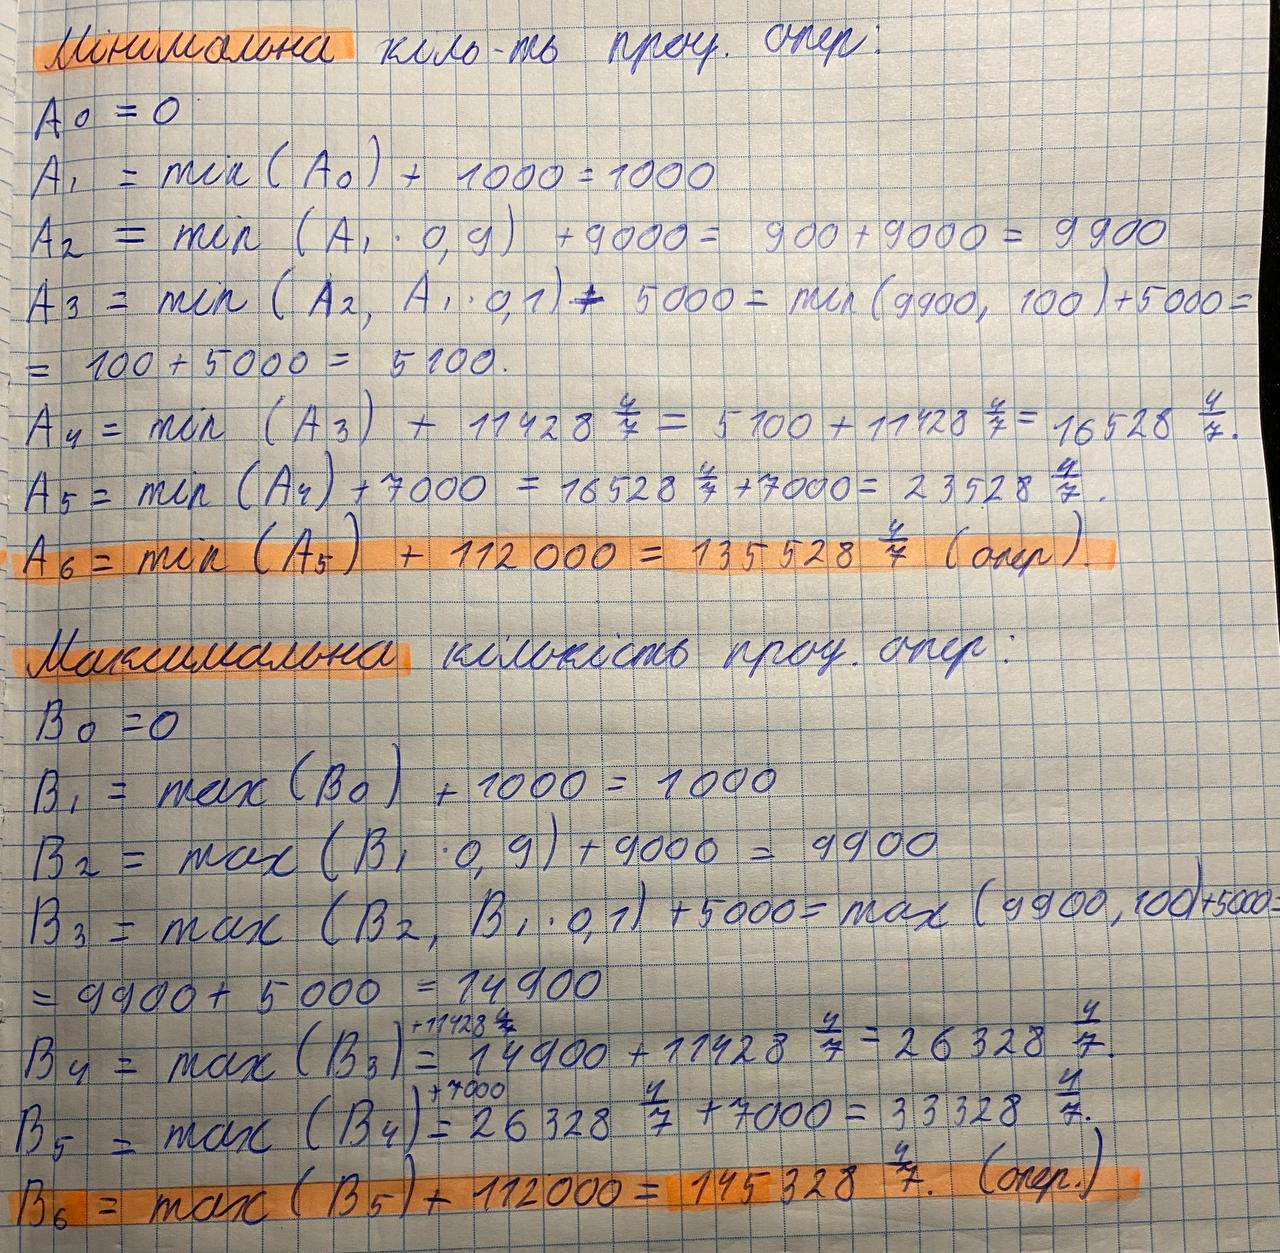
\includegraphics[width=14cm]{reports/algos/lab1/assets/12.jpg}
    \caption{Мінімальна та максимальна трудомісткість}
\end{figure}

\section{Висновки}
В ході виконання я лабораторної роботи я розрахував трудомісткість алгоритму двома різними методами: методом теорії марковських ланцюгів та мережевим методом. Результати розрахунку середньої кількості процесорних операцій, що визначена із використанням \textbf{стохастичної матриці} та \textbf{алгоритму мережевого підходу}, збіглися. \\

    При обчисленні \textbf{максимальної} та \textbf{мінімальної} кількості операцій алгоритму, я отримав значення мінімальної яка \textbf{менша} за середню трудомісткість, та значення максимальної яка \textbf{більша} за середню трудомісткість, це значить що мої розрахунки повністю вірні.